\chapter{Design and Implementation}
\label{chap:design_and_implementation}


\section{Introduction}
In this chapter, we will discuss the design and implementation of the \ac{POP} algorithm.
We will start by discussing the design of the algorithm,
and then we will discuss the implementation of the algorithm in C\#.

\section{Design of the Algorithm \& Class Diagram}
\subsection{Nondeterministic Achievers \& Threat Search}
\acf{POP} needs to be able to handle some form of nondeterminism in the planning domain. This is because the planner needs
to be able to handle situations where there are multiple ways to achieve a precondition
of an action. This cannot be achieved in practice without trying to search all possible ways of the choices that can be made.
So, to model nondeterminism in the planning domain, we need to introduce the concept of \textbf{A* Search}.
A* Search is a search algorithm that is


% put the image of the class diagram here (POP.png)
\begin{figure}[ht]
    \centering
    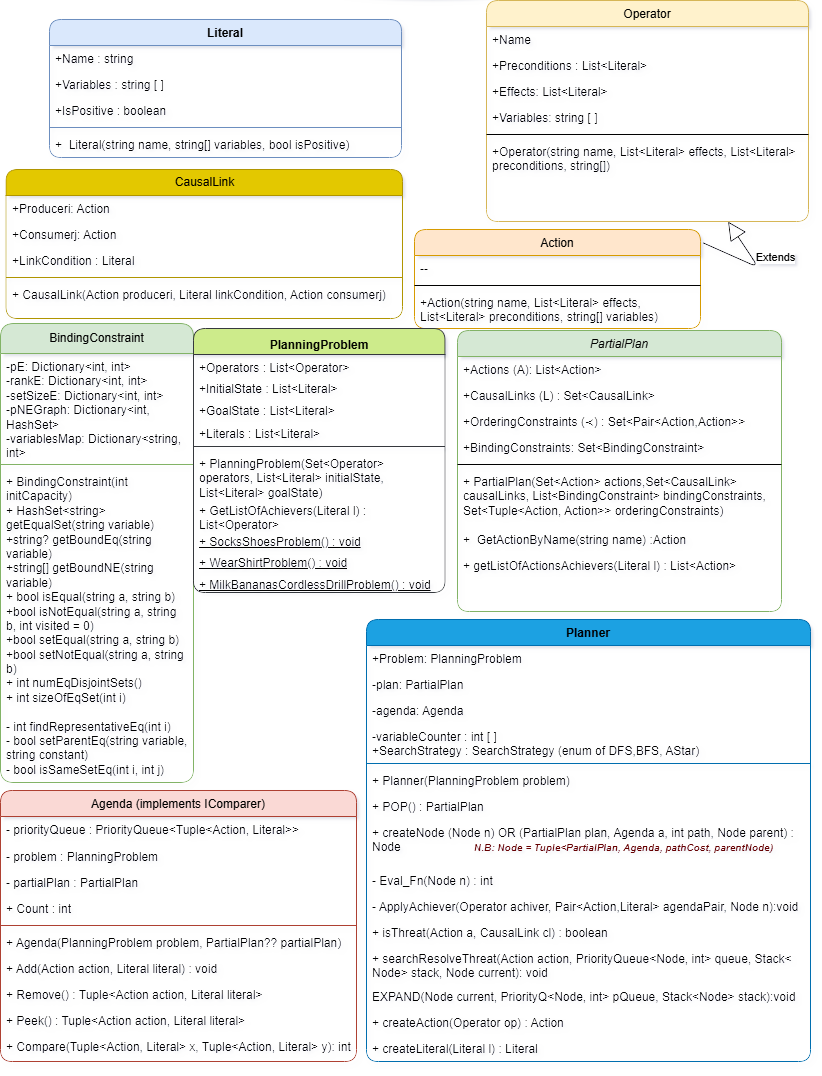
\includegraphics[width=0.9\textwidth]{images/POP.png}
    \caption[Class Diagram of the POP Algorithm]{Class Diagram of the POP Algorithm}
    \label{fig:pop}
\end{figure}